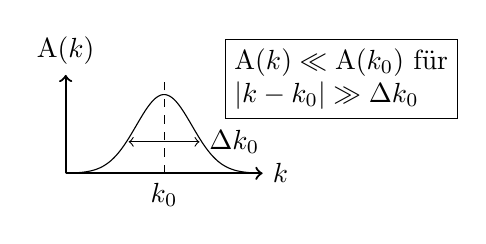
\begin{tikzpicture}[scale=0.5, samples=200, domain=0:5]
	% Achsen zeichnen
	\draw[->,thick] (0,0) -- (5,0) node[right] {$ k$};
	\draw[->,thick] (0,0) -- (0,2.5) node[above] {$\mathrm{A}( k)$};
	%Plot
	\draw plot (\x,{exp(-(\x-2.5)^2)*2});
	\draw [style=dashed] (2.5,0) node[below] {$ k_0$} --(2.5,2.4);
	\draw[<->] (1.6,.8)--(3.4,.8) node[right] {$\Delta  k_0$};
	\node[draw,align=left] at (7,2.4) {$\mathrm{A}( k) \ll \mathrm{A}( k_0)$ für\\ $| k- k_0| \gg \Delta  k_0$};
\end{tikzpicture}